\documentclass[10pt]{book} 
\usepackage[width=5in, height=3in]{geometry} 
\usepackage{amsmath, amsfonts, amssymb}
\usepackage{physics}
\usepackage{mathptmx}

\usepackage{lipsum}
\usepackage{multicol}
\usepackage{xcolor}
\usepackage{soul}
\sethlcolor{yellow}
\pagestyle{empty}
\newcommand{\unit}[1]{\mathrm{#1}}
\newcommand{\E}[2]{\times10^{#1}\,\unit{#2}}

\usepackage{tcolorbox}
\tcbuselibrary{poster}
\usepackage{graphicx} %%Insert filepath
	\graphicspath{ {./images/} }

\begin{document}

\begin{tcbposter}[
  poster = {%showframe,
    columns=3,
    rows=1,
    spacing=1mm,
  },
]

\posterbox[
top=1pt,
bottom=1pt,
left=1pt,
right=1pt,
tile,
colback=white,
]{
  name=Col,
  sequence = 1 between top and bottom then
             2 between top and bottom then
             3 between top and bottom,
}{
  \tiny
  \hl{TEST 1}\\
  \textbf{Laplace Transform} \\
\textit{a)} \ $F(s)= \int_{o}^{\infty} f(t) e^{-st}$ \\
\textit{b)} \ Integrate, remove any u(t). Only values on the positive side of 
x-axis are important. Remove u(t), change integral limits.\\
\textit{c)}\ Linearity: $c_1f_1(t)+c_2f_2(t) = c_1F_1(s)+c_2F_2(s)$ \\
\textit{d)}\ Time Shift: $f(t-t_o)u(t-t_o) = e^{-st_{o}}F(s)$ \\
\textit{d)}\ IVT: Multiply by s first. If $\frac{\infty}{\infty}$, divide top and bottom by s. Solve for $s = \infty$.\\
\textit{e)}\ FVT: Multiply by s first. Solve for $s = 0$. \\
\textit{f)}\ Unit Step: Unit step is the integral of the unit sample. The 
unit sample is the derivative of the unit step. 

	\textbf{Inverse Laplace}\\
\textit{1.a)} Standard form: decreasing powers of s, coefficient of largest power in den = 1. \\
\textit{1.b)} Make Ratio Proper: Power of s in num must be less than or equal to den. If not true, use long division. \\
\textit{1.c)} Find Poles (roots of den): Factor or use quadratic formula. Roots can be real/unique, real/repeated, or complex/unique. Real parts for roots should be less than or equal to 0. \\
\textit{1.d)} Break Into Sums: \\
For real/unique, use sums of $\frac{A}{(s+k)} + \frac{B}{(s+k)}$ ... \\
For real/repeated, use sums of $\frac{A}{(s+k)^2} + \frac{B}{(s+k)}$ ... \\
For every complex/unique, $s = - \alpha +- j \omega $  and do the sums of
$\frac{A}{s+ \alpha - j \omega} + \frac{A^*}{s+ \alpha + j \omega}$. For calc use 
cSolve(blah+x=0,x) to get complex roots.\\
\\
\\
\\
\\
\\
\\
\textit{1.e)} Solve A, B, C... \\
 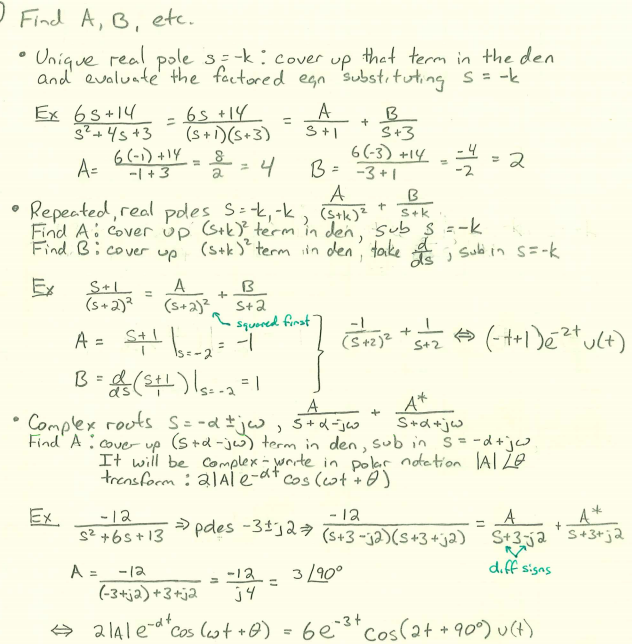
\includegraphics[scale=0.314]{note1.png}\\
 
	\textbf{Convolution}\\
\textit{2.a)} $y(t)= \int_{-\infty}^{\infty} x(\tau)h(t-\tau)d\tau = x(t) * h(t)$ \\
\textit{2.b)} Get rid of u(t). Great new piece-wise function for t $\geqslant$ 0 and t 
$\leqslant$ 0.\\
\textit{2.c)} Can be replaced by Laplace, via Y(s) = X(s)H(s). Then follow 
\textit{1.a} to \textit{1.e}.\\
\\
\\
\\
\\
\\
\\
	\textbf{Circuit Elements and Laplace} \\
\textit{3.a) }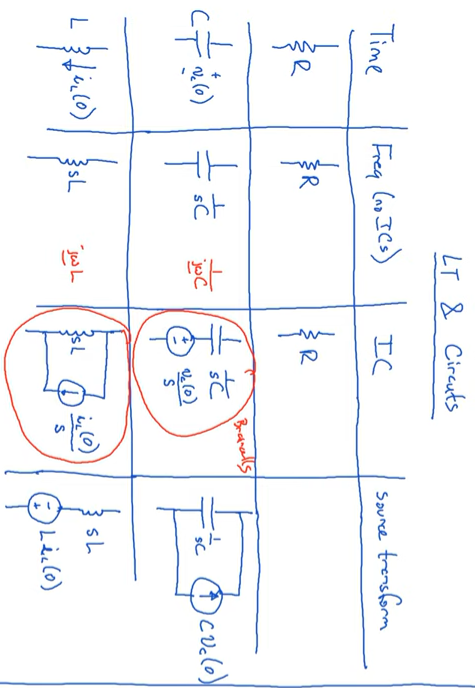
\includegraphics[scale=0.36]{note2.png}\\
\textit{3.b) } Transform the circuit to the frequency domain.\\
\textit{3.c) } Use nodal or mesh to solve given problem.\\
\textit{3.d) } Reduce and the perform inverse Laplace transform.\\



  


   }
\end{tcbposter}
\noindent
\begin{tcbposter}[
  poster = {%showframe,
    columns=3,
    rows=1,
    spacing=1mm,
  },
]
\noindent
\posterbox[
top=1pt,
bottom=1pt,
left=1pt,
right=1pt,
tile,
colback=white,
]{
  name=Col,
  sequence = 1 between top and bottom then
             2 between top and bottom then
             3 between top and bottom,
}{
  \tiny
  \hl{TEST 2}\\
  
}
\end{tcbposter}

\end{document}